\documentclass{beamer}


% Load essential packages
\usepackage{hyperref} % Only load once to avoid conflicts
\usepackage{stile}
\usepackage{subcaption}
\usepackage{tcolorbox}
\usepackage[font=scriptsize,skip=1pt]{caption}
\usepackage[T1]{fontenc}
\usepackage{csquotes}
\usepackage[backend=biber, style=authoryear, maxnames=3, minnames=1, abbreviate=false, date=long, url=false, isbn=false, doi=false]{biblatex}
\addbibresource{lecture10/bib.bib} % Ensure this matches your bibliography file name

\interfootnotelinepenalty=10000

\usepackage{latexsym, amsmath, xcolor, multicol, booktabs, calligra}
\usepackage{graphicx, pstricks, listings, stackengine}

% Hyperref setup
\hypersetup{
    hidelinks,
    colorlinks=true,
    linkcolor=black,
    citecolor=blue,
    urlcolor=black
}

% Font theme for Beamer
\usefonttheme[onlymath]{serif}

% Custom definitions
\def\cmd#1{\texttt{\color{red}\footnotesize $\backslash$#1}}
\def\env#1{\texttt{\color{blue}\footnotesize #1}}
\definecolor{deepblue}{rgb}{0,0,0.5}
\definecolor{deepred}{rgb}{0.6,0,0}
\definecolor{deepgreen}{rgb}{0,0.5,0}
\definecolor{halfgray}{gray}{0.55}

% Beamer color settings
\setbeamercolor{block title}{bg=blue!70!white, fg=white}
\setbeamercolor{block body}{bg=blue!10!halfgray, fg=white}
\setbeamercolor{section in head/foot}{fg=white}
\setbeamercolor{subsection in head/foot}{fg=white}
\setbeamercolor{title in head/foot}{fg=white}


% Listings settings for code highlighting
\lstset{
    basicstyle=\ttfamily\small,
    keywordstyle=\bfseries\color{deepblue},
    emphstyle=\ttfamily\color{deepred},
    stringstyle=\color{deepgreen},
    numbers=left,
    numberstyle=\small\color{halfgray},
    rulesepcolor=\color{red!20!green!20!blue!20},
    frame=shadowbox,
}

% Title page info
\author{Freya Rubel}
\title{Trade, Migration and Global Challenges}
\subtitle{Populism}
\institute{}
\date{08.01.2026}

\graphicspath{{lecture10/}}

\begin{document}

\begin{frame}
    \titlepage
\end{frame}

\begin{frame}
    \tableofcontents[sectionstyle=show, subsectionstyle=show/shaded/hide, subsubsectionstyle=show/shaded/hide]
\end{frame}


\section{Introduction}

\begin{frame}{Defining Populism}
Populism divides society into two groups:
\begin{center}
\textbf{"The pure people"} vs. \textbf{"The corrupt elite"}
\end{center}
\vspace{0.3cm}
Key characteristics:
\begin{itemize}
    \item Anti-establishment rhetoric attacking elites, intellectuals, and institutions
    \item Claims of perpetual crisis
    \item Populists are "the voice of the people" - anti-pluralism
    \item Combined with other ideologies: nationalism, socialism, or libertarianism
\end{itemize}
\vspace{0.3cm}
\textit{Note}: Populism is an analytical category, not a value judgment. Related concept: \textit{demagogy} refers to politics that offers overly simplistic answers to complex problems, typically in an emotional manner.
\end{frame}

\begin{frame}{A Historical Pattern}
Populism isn't new. Previous waves of globalization triggered populist backlashes:
\begin{itemize}
\item \textbf{1890s US Populist Party}: Farmers faced falling crop prices due to global competition and demanded: (1) expanding the money supply to create inflation and reduce their debt burdens, and (2) regulation of railroad monopolies that charged high rates to transport crops to market.
    \item \textbf{1930s Europe}: Economic depression and trade collapse contributed to the rise of fascist movements with populist and anti-establishment rhetoric.
\item \textbf{Today}: Post-1990s hyperglobalization met renewed populist movements, with today's populism centering on manufacturing decline and urban-rural divides in post-industrial economies.
\end{itemize}
\end{frame}


\begin{frame}{Why This Matters}
Populist movements are able to mobilise voters and shape policy outcomes through:
\begin{itemize}
    \item Trade agreements
    \item Immigration policy
    \item International cooperation
    \item Domestic redistribution
\end{itemize}
\vspace{0.5cm}
Understanding what drives populism helps us understand the political sustainability of globalization and potential policy responses.
\end{frame}

\begin{frame}{The Rise and Fall of Populism - Visual Evidence}
    \begin{figure}
        \centering
        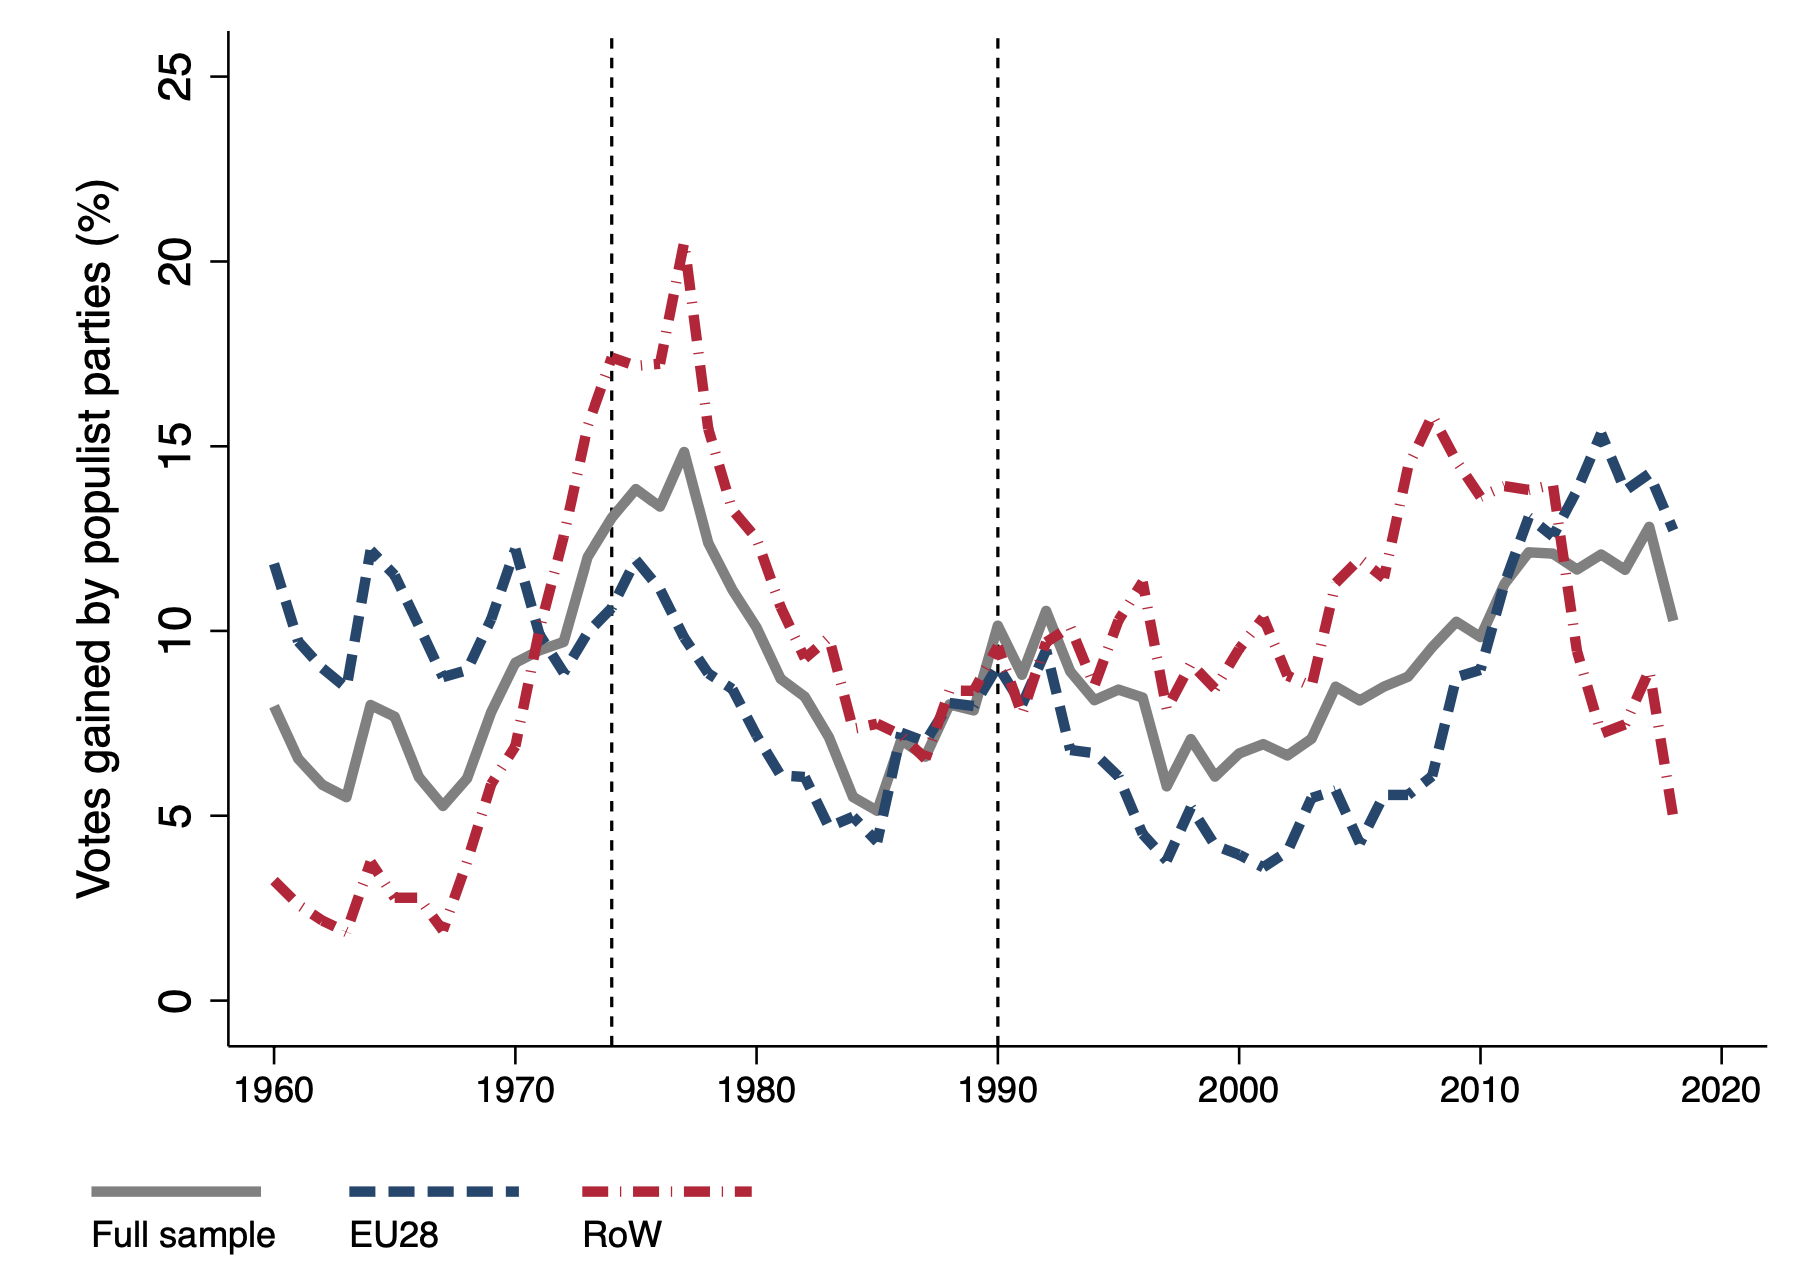
\includegraphics[width=0.8\linewidth]{vote share gained by populists.png}
        \caption{Source: \textcite{globalization_and_populism}}
    \end{figure}
\end{frame}


\section{Measuring Populism}

\begin{frame}{Measuring Populism - Why It's Challenging}
Traditional approach: Binary classification of parties as "populist" or not, then sum their vote share.
\vspace{0.3cm}

\textbf{Limitations}:
\begin{itemize}
    \item All populist parties treated equally (ignores intensity)
    \item Doesn't capture mainstream parties adopting populist rhetoric
    \item Classification depends on the individual country's baseline level of populism in politics
\end{itemize}
\vspace{0.3cm}
$\rightarrow$ We need better measures to understand what's actually driving the phenomenon.
\end{frame}

\begin{frame}{A Different Measurement Approach}
Party-level populism score with two dimensions:
\vspace{0.3cm}

\textbf{1. Anti-Establishment Stance (AES)}
\begin{itemize}
    \item Emphasis on eliminating corruption
    \item Anti-pluralism (others lack competence)
\end{itemize}
\vspace{0.3cm}
\textbf{2. Commitment to Protect (CTP)}
\begin{itemize}
    \item Internal market protection
    \item Opposition to internationalism
    \item Opposition to international institutions
    \item Support for nationalization
\end{itemize}
\vspace{0.3cm}
Scores derived from party manifestos: what parties declare to do if in power.
\end{frame}

\begin{frame}{Populism Intensity Over Time}
    \begin{figure}
        \centering
        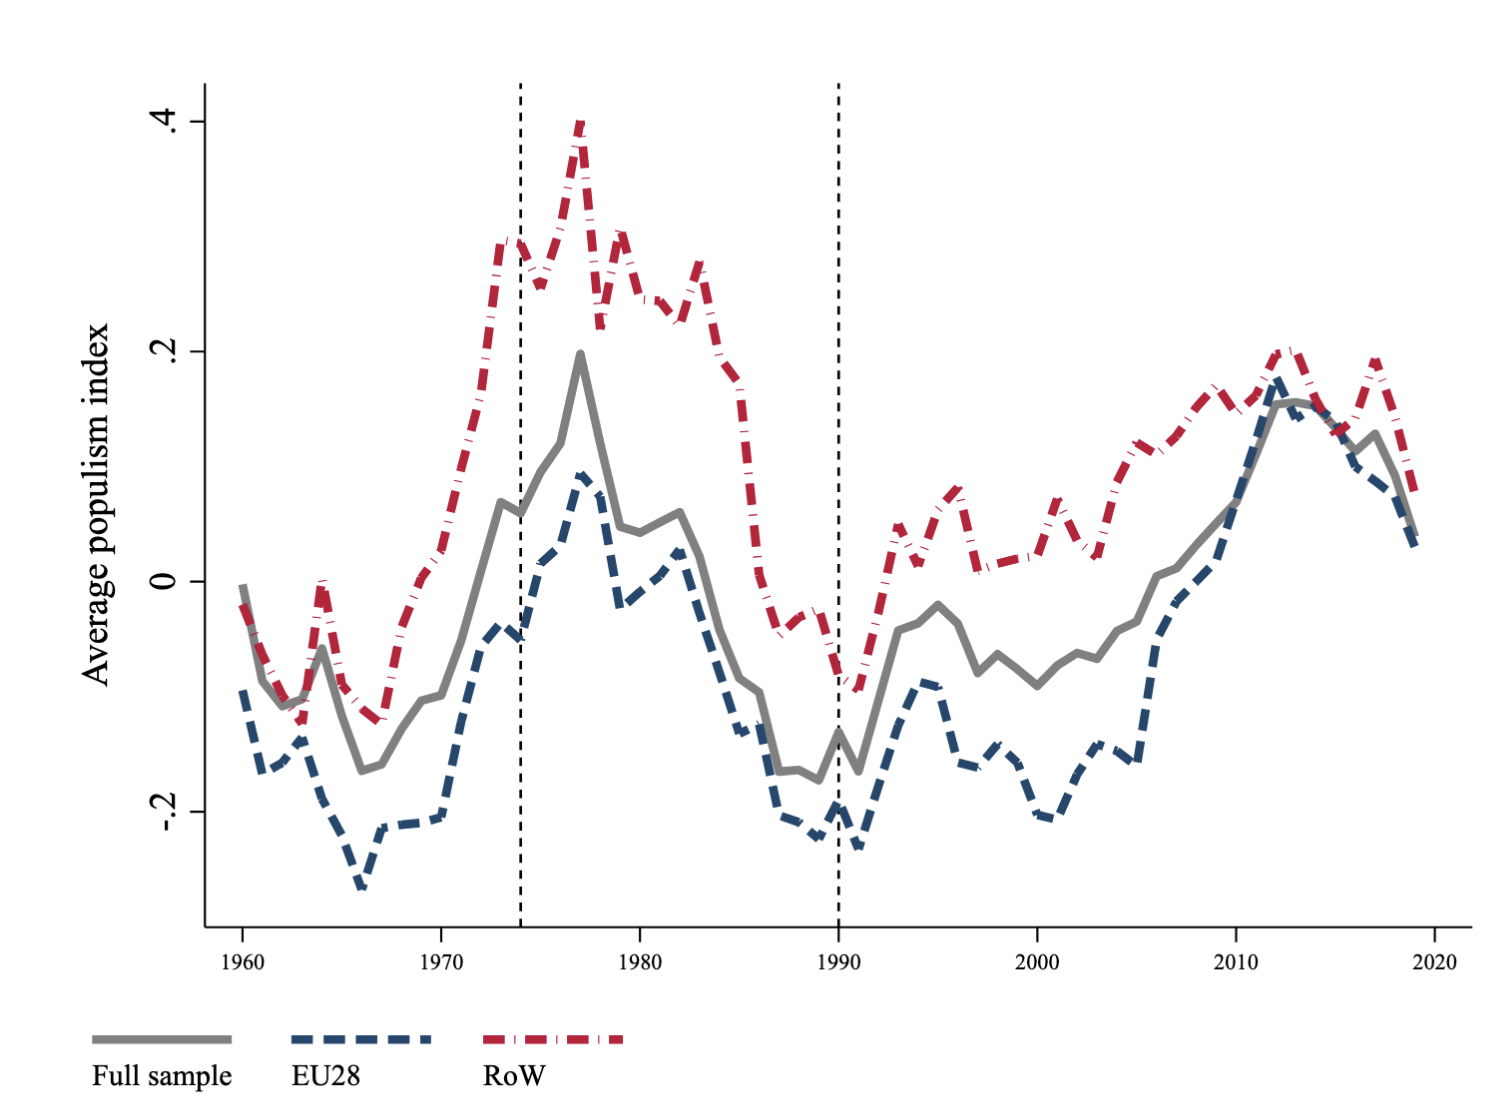
\includegraphics[width=0.8\linewidth]{populism_intensity_unweighted.png}
        \caption{Source: \textcite{globalization_and_populism}}
    \end{figure}
\end{frame}

\section{Channels and Mechanisms}

\begin{frame}{The Central Puzzle}
\textbf{Observation}: Globalization has accelerated since 1990. Populism has risen since 1990.
\vspace{0.5cm}

\textbf{Questions}:
\begin{itemize}
    \item Is this correlation causal?
    \item What are the mechanisms linking globalization to populism?
    \item Why has the response been predominantly right-wing when left-wing movements have redistributive agendas that should appeal to globalization's losers?
\end{itemize}
\end{frame}

\begin{frame}{Two Sides of Political Competition}
  \begin{figure}
      \centering
      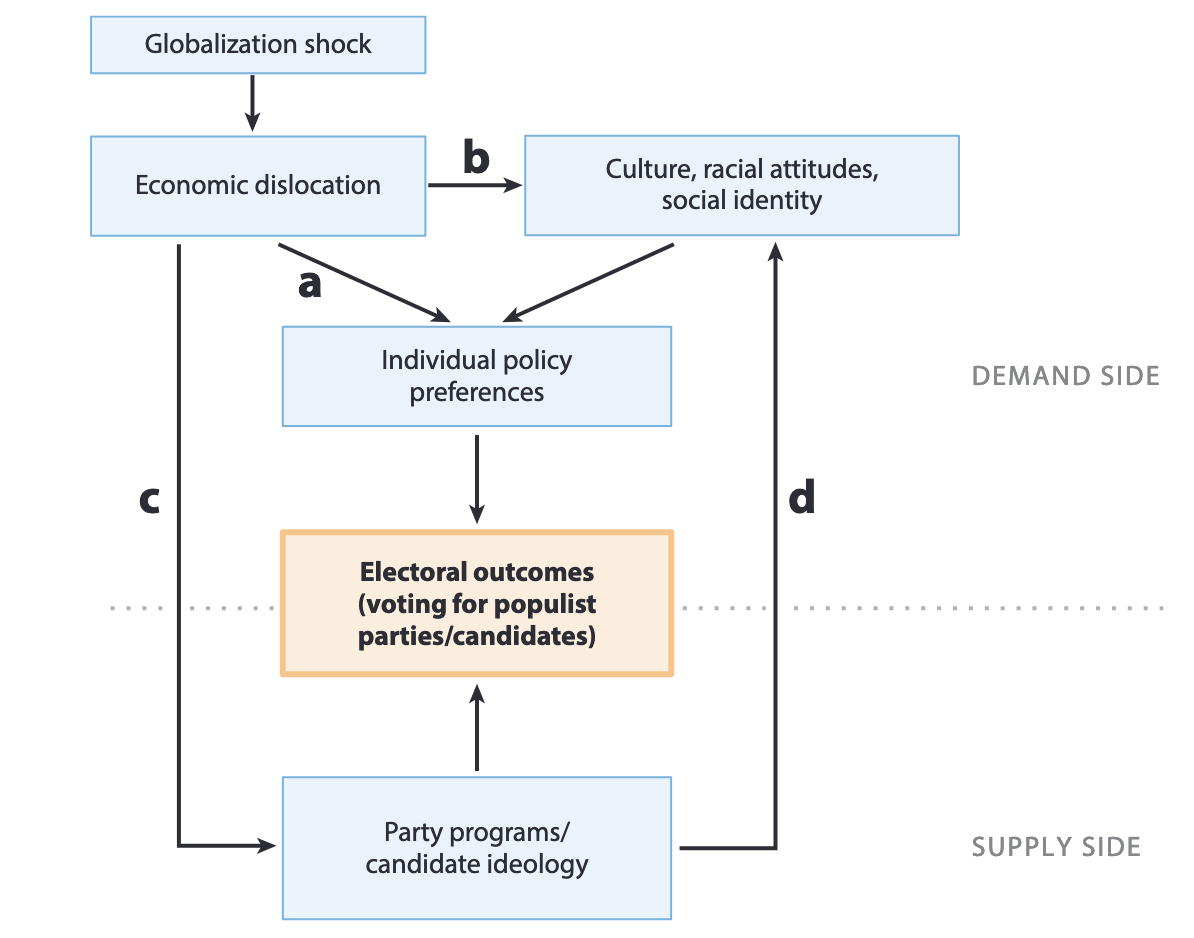
\includegraphics[width=0.7\linewidth]{Bildschirmfoto 2024-12-18 um 14.55.16.png}
      \caption{Source: \textcite{rodrik_annual_reviews_populism_globalization}}
  \end{figure}
  \vspace{0.3cm}
  %\textbf{Demand side}: What voters want (preferences shaped by economic conditions, identity, values)
  
  %\textbf{Supply side}: What parties offer (platforms, candidates, strategic positioning)
  
  %Globalization can affect both sides.
\end{frame}

\begin{frame}{Channel A - Direct Economic Preferences}
\textbf{Mechanism}: Economic dislocation directly shapes policy preferences.
\vspace{0.3cm}

\textbf{Example}: 
\begin{itemize}
    \item Region experiences manufacturing job losses due to import competition
    \item[$\rightarrow$] Workers face unemployment or wage decline
    \item[$\rightarrow$] Voters support protectionist policies and anti-globalization candidates
\end{itemize}
\vspace{0.3cm}
This is the most intuitive channel: pocketbook voting.
\end{frame}

\begin{frame}{Channel B - Identity and Cultural Values}
\textbf{Mechanism}: Economic shocks reshape identity and cultural attitudes.
\vspace{0.3cm}

\textbf{Example}: 
\begin{itemize}
    \item Economic insecurity $\rightarrow$ threat of own identity (as middle-class American)
    \item[$\rightarrow$] Nostalgia for past stability
    \item[$\rightarrow$] Emphasis on traditional values and local identity
    \item[$\rightarrow$] Stronger "us vs. them" distinction
\end{itemize}
\vspace{0.3cm}
Cultural politics can have economic roots. The key question: Is this truly about culture, or economics disguised in cultural language?
\end{frame}

\begin{frame}{Channel C - Party Positioning}
\textbf{Mechanism}: Economic shocks shift party priorities.
\vspace{0.3cm}

\textbf{Example}: 
\begin{itemize}
    \item Import competition harms manufacturing workers
    \item[$\rightarrow$] Parties adopt more protectionist positions to capture these voters
    \item[$\rightarrow$] Political spectrum becomes more polarized on trade
\end{itemize}
\vspace{0.3cm}
Even if voter preferences were to remain constant, they face different policy choices because parties have repositioned. % this is especially critical if you have a two party system. If there are only two choices and they position themselves at opposite poles, there is a good chance that you agree with neither of them 
\end{frame}

\begin{frame}{Channel D - Strategic Framing}
\textbf{Mechanism}: Parties strategically emphasize certain issues to win.
\vspace{0.3cm}

\textbf{Example}: 
\begin{itemize}
    \item Right-wing party loses median voter support due to economic inequality % globalization typically increases economic inequality (income inequality) and the econimic response should be stronger redistriction, which is a typical left policy
    \item[$\rightarrow$] Party shifts focus from economic to cultural issues (immigration, identity)
    \item[$\rightarrow$] Low-income voters support party based on cultural alignment despite the fact that they don't represent their best economic interests
\end{itemize}
\end{frame}

\begin{frame}{The Skill Dimension}
Not all globalization is the same. The skill content of imports and immigration determines which populists win and lose:
\vspace{0.3cm}

\textbf{Low-skill imports}: Compete with domestic low-skill workers $\rightarrow$ downward wage pressure $\rightarrow$ demand for protection
\vspace{0.3cm}

\textbf{High-skill imports}: Suggest comparative advantage and specialization $\rightarrow$ complementary to domestic production $\rightarrow$ less threatening
\vspace{0.3cm}

Same logic applies to immigration. This distinction is crucial for understanding heterogeneous political responses.
\end{frame}

\section{Empirical Evidence}

\begin{frame}{Trump Voters in 2016}
\textcite{rodrik_annual_reviews_populism_globalization} conducts a survey of US electorate (N=885) comparing Trump vs. Clinton voters:
\vspace{0.3cm}

\textbf{Trump voters (on average)}:
\begin{itemize}
    \item Opposed free trade agreements and immigration
    \item Identified with upper social class
    \item Did not express economic worries
    \item Displayed higher racial hostility
\end{itemize}
\end{frame}

\begin{frame}{The Switchers Matter}
\textbf{Obama 2012 $\rightarrow$ Trump 2016 switchers} were different:
\vspace{0.3cm}

\textbf{Economic characteristics}:
\begin{itemize}
    \item Did NOT identify with upper social class
    \item Expressed financial worries
\end{itemize}
\vspace{0.3cm}
\textbf{Attitudes}:
\begin{itemize}
    \item Disliked trade and immigration (like Trump voters)
    \item More racially hostile than average Obama voters
\end{itemize}
\vspace{0.3cm}
These marginal voters (those who actually shifted the outcome) show both economic and cultural motivations for their shift towards a populist.
\end{frame}

\begin{frame}{Comparative Evidence Across Democracies}
\textcite{globalization_and_populism}: 628 elections in 55 countries over 60 years
\vspace{0.3cm}

\textbf{Data advantages}:
\begin{itemize}
    \item Long time span captures multiple globalization waves
    \item Cross-country variation in exposure to trade/migration
    \item Measures both vote share and populism intensity
\end{itemize}
\vspace{0.3cm}
\textbf{Key innovation}: Distinguishes skill content of imports and immigration to test mechanisms of high vs. low skill globalization.
\end{frame}

\begin{frame}{Effect of Low-Skill Import Competition}
\textbf{Imports of low-skill labor-intensive goods}:
\vspace{0.3cm}

\textit{Vote share effects}:
\begin{itemize}
    \item[$\uparrow$] Right-wing populist vote share
    \item[$\uparrow$] Left-wing populist vote share
\end{itemize}
\vspace{0.3cm}
\textit{Populism intensity}:
\begin{itemize}
    \item[$\uparrow$] Right-wing populism score
    \item No effect on left-wing populism score
\end{itemize}
\vspace{0.3cm}
Right-wing populist parties don't just gain votes - they become more populist in rhetoric and platform.
\end{frame}

\begin{frame}{Effect of High-Skill Import Competition}
\textbf{Imports of high-skill labor-intensive goods}:
\vspace{0.3cm}

\textit{Vote share effects}:
\begin{itemize}
    \item[$\downarrow$] Right-wing populist vote share
    \item No effect on left-wing populist vote share
\end{itemize}
\vspace{0.3cm}
\textit{Populism intensity}:
\begin{itemize}
    \item[$\downarrow$] Right-wing populism score (if any effect)
\end{itemize}
\vspace{0.3cm}
High-skill imports are associated with less populism, consistent with complementarity and shared gains.
\end{frame}

\begin{frame}{Effect of Low-Skill Immigration}
\textbf{Immigration of low-skilled labor}:
\vspace{0.3cm}

\textit{Vote share effects}:
\begin{itemize}
    \item[$\uparrow$] Right-wing populist vote share
    \item[$\downarrow$] Left-wing populist vote share
\end{itemize}
\vspace{0.3cm}
\textit{Populism intensity}:
\begin{itemize}
    \item No detectable effect
\end{itemize}
\vspace{0.3cm}
Low-skill immigration benefits right-wing populists specifically, potentially because they can frame it as cultural threat alongside economic competition. Voters shift from left-wing populists to right-wing populists.
\end{frame}

\begin{frame}{Effect of High-Skill Immigration}
\textbf{Immigration of high-skilled labor}:
\vspace{0.3cm}

\textit{Vote share effects}:
\begin{itemize}
    \item[$\downarrow$] Right-wing populist vote share
    \item[$\uparrow$] Left-wing populist vote share
\end{itemize}
\vspace{0.3cm}
\textit{Populism intensity}:
\begin{itemize}
    \item No detectable effect
\end{itemize}
\vspace{0.3cm}
High-skill immigration may be seen as benefiting elites/corporations, creating opportunity for left-wing critique.
\end{frame}

\begin{frame}{When Do These Effects Get Amplified?}
Testing for conditions that strengthen the relationship between globalization and populism:
\vspace{0.3cm}

\textbf{Potential amplifiers}:
\begin{itemize}
    \item Economic crisis (negative income growth)
    \item De-industrialization (manufacturing share declining)
    \item Social media prevalence (internet coverage)
    \item Diversity of import origins
    \item Cultural distance between natives and migrants
\end{itemize}
\end{frame}

\begin{frame}{Economic Amplifiers}
    \begin{figure}
        \centering
        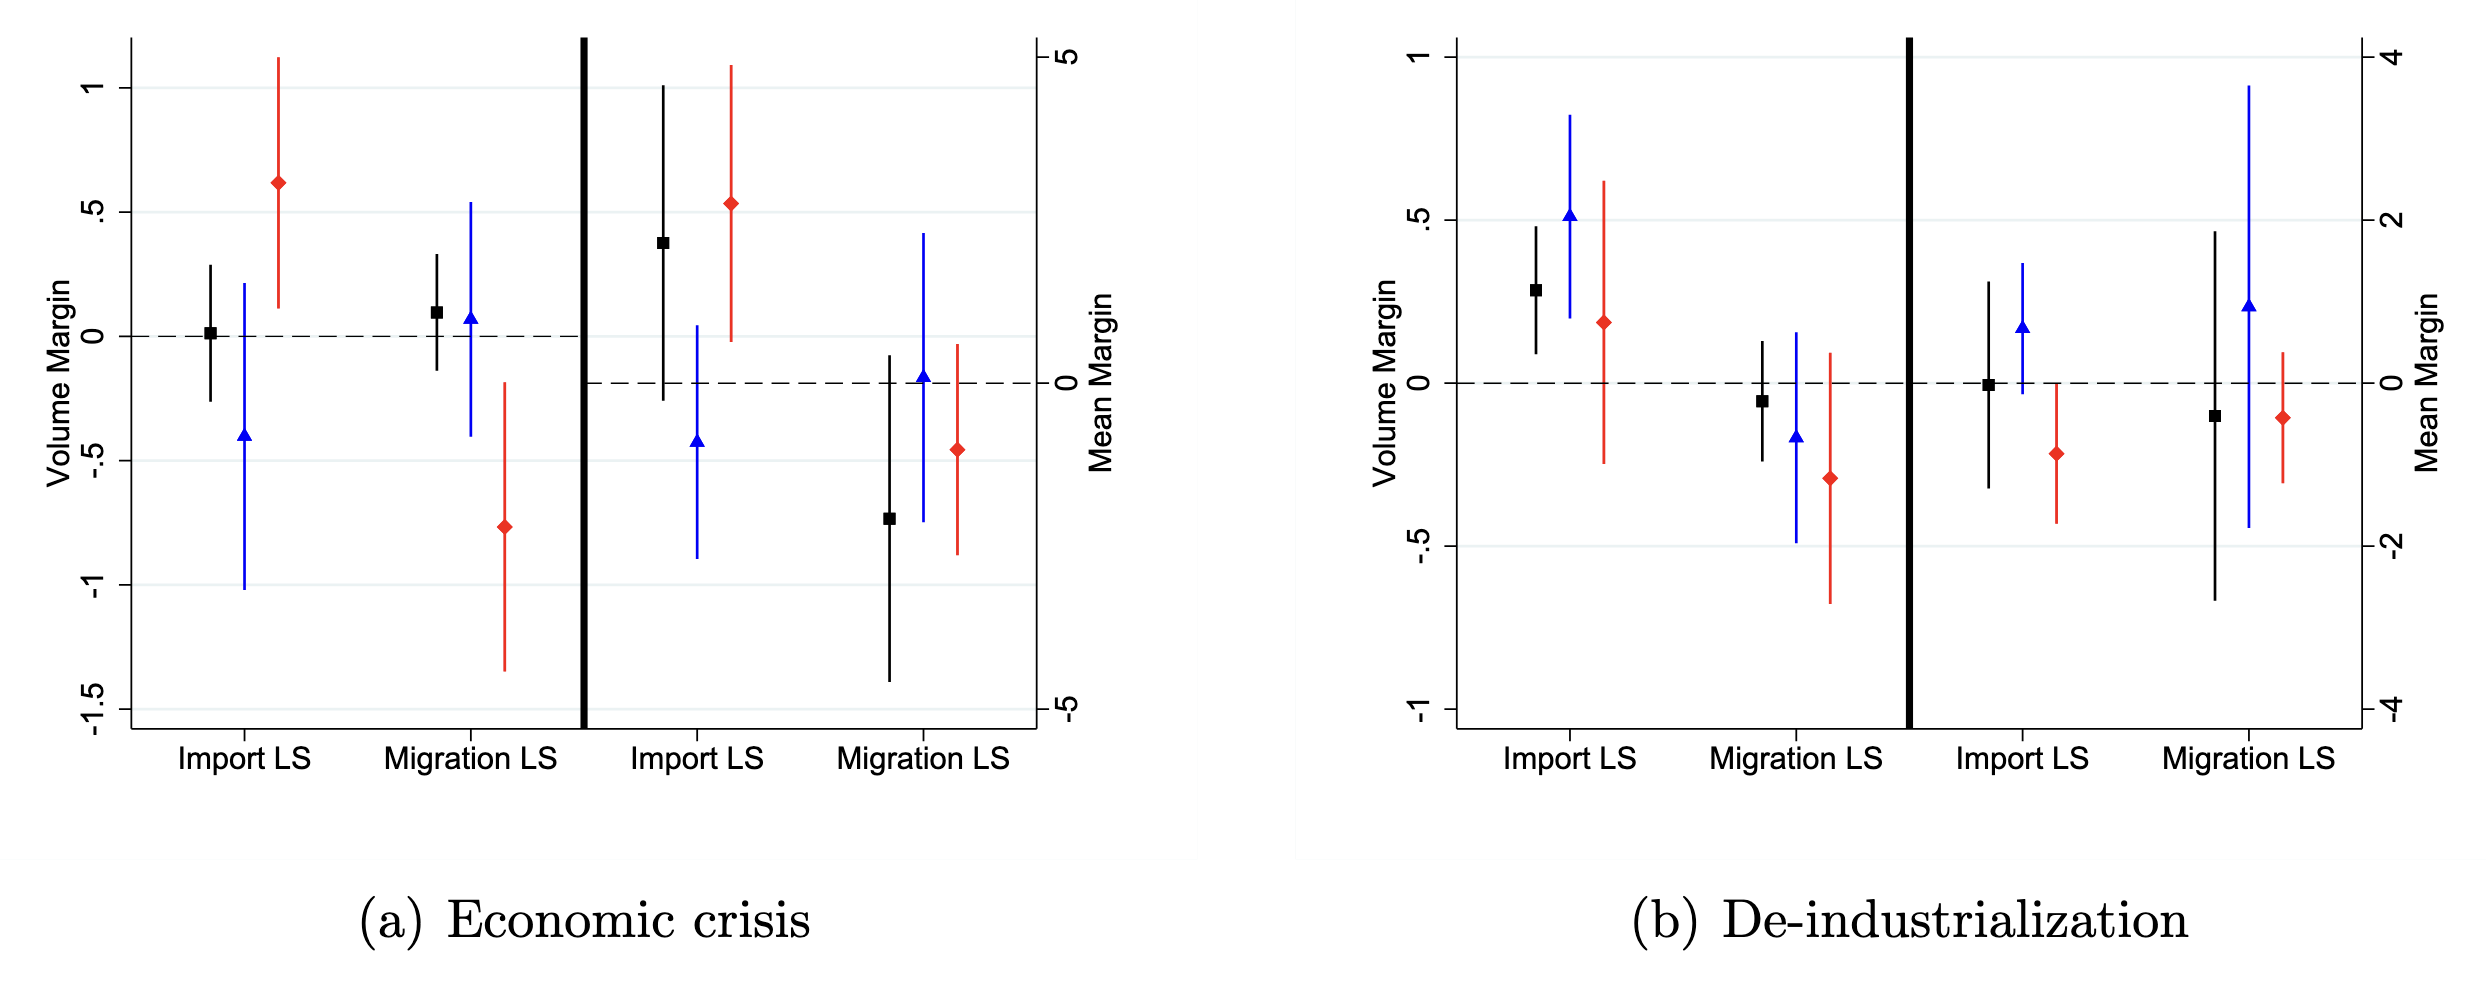
\includegraphics[width=\linewidth]{economic amplifiers.png}
        \caption{Point estimates with 90\% confidence intervals. Blue = right-wing, Red = left-wing. Source: \textcite{globalization_and_populism}}
    \end{figure}
    \textbf{Key findings}: De-industrialization amplifies the right-wing populist response to low-skill imports. Economic crisis amplifies left-wing populist response to low-skill imports.
\end{frame}

\begin{frame}{Media and Diversity Amplifiers}
    \begin{figure}
        \centering
        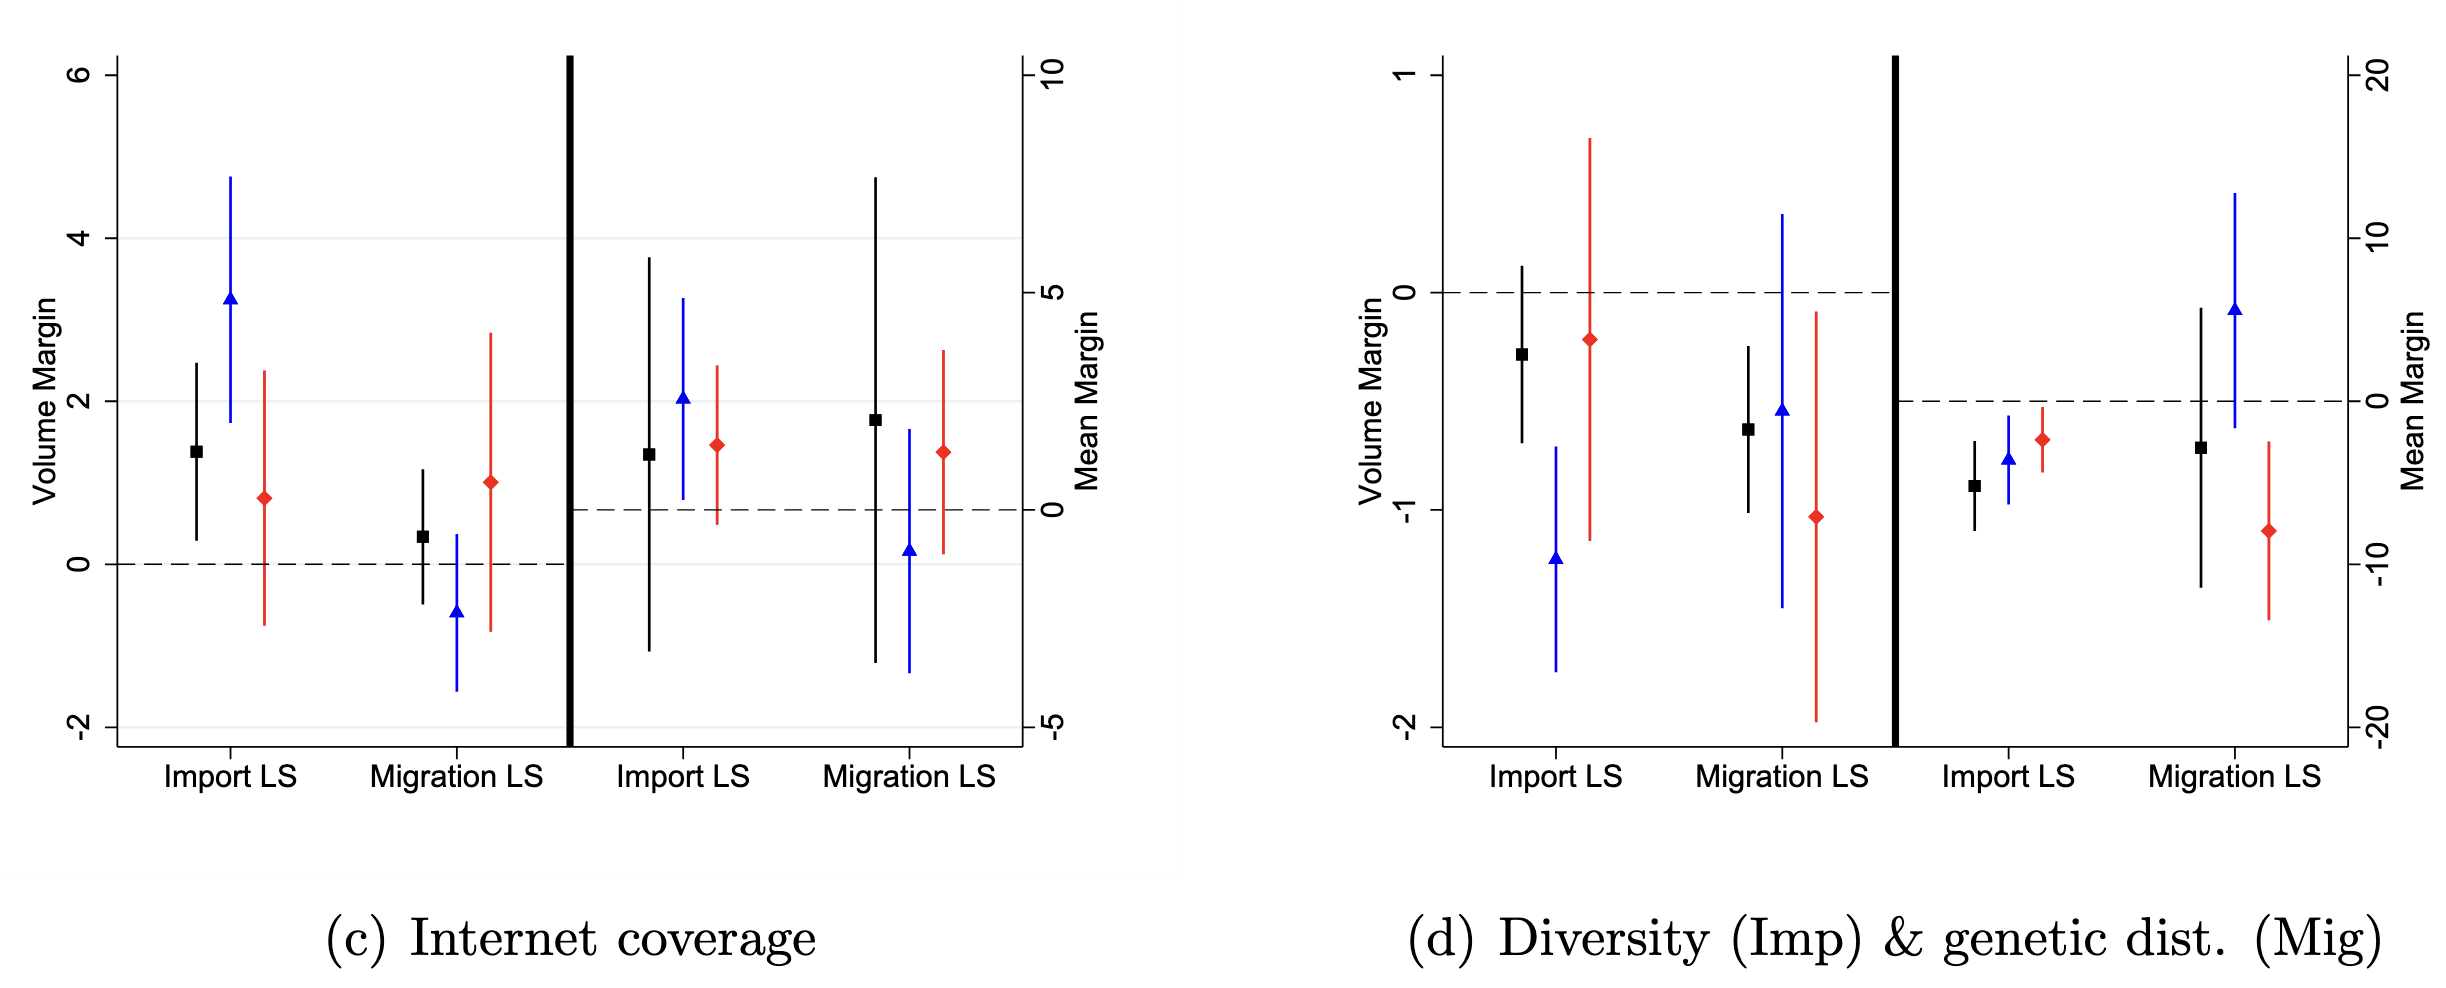
\includegraphics[width=\linewidth]{media and diversity amplifiers.png}
        \caption{Point estimates with 90\% confidence intervals. Blue = right-wing, Red = left-wing. Source: \textcite{globalization_and_populism}}
    \end{figure}
    \textbf{Key findings}: High internet coverage amplifies right-wing populist response (both volume and intensity). Greater diversity in import origins reduces right-wing populist response.
\end{frame}

\begin{frame}{The Social Media Mechanism}
Why does internet coverage specifically amplify populism?
\vspace{0.3cm}

\textbf{Hypotheses}:
\begin{itemize}
    \item Direct communication bypassing traditional media gatekeepers
    \item Echo chambers reinforcing own beliefs about the world
    \item Viral emotional content over nuanced policy debate
\end{itemize}
\vspace{0.3cm}
This deserves more research, but the amplification effect is substantial.
\end{frame}


\begin{frame}{The Right-Wing Advantage}
Why has populism been predominantly right-wing despite economic arguments favoring left-wing redistribution?
\vspace{0.3cm}

\textbf{Geographic sorting}: Less educated, socially conservative voters concentrated in economically declining areas. Urban areas benefit from globalization, creating spatial polarization.
\vspace{0.3cm}

\textbf{Strategic framing}: Right-wing parties leverage identity issues (race, immigration, traditional values) to attract economically struggling voters. When inequality rises, parties representing the wealthy have incentive to shift discourse from economics to culture.
\vspace{0.3cm}

\textbf{Result}: Economic hardship + cultural division = powerful mobilization tool for right-wing populists.
\end{frame}

\begin{frame}{Are Populists Always Protectionist?}
\textbf{Brexit case}: British populists supported leaving the EU partly to enable \textit{more} free trade.
\vspace{0.3cm}

\textbf{Argument}: EU was protectionist bloc (agricultural tariffs, manufacturing protection). Brexit would mean bilateral trade deals and lower barriers.
\vspace{0.3cm}

\textbf{Lesson}: Populists oppose \textit{elites} (domestic or international) who undermine popular will. In 1890s America, populists wanted free trade because protection helped elites. Today's populists want protection because globalization helps elites.
\vspace{0.3cm}

The target is elite power, not trade per se.
\end{frame}


\begin{frame}{Discussion Questions}
\begin{enumerate}
    \item The evidence shows low-skill import competition increases populism. Does this mean countries should restrict such imports? What are the tradeoffs?
    \vspace{0.3cm}
    \item If economic insecurity drives cultural backlash (Channel B), should policy focus on economic support or cultural integration? Can you address one without the other?
    \vspace{0.3cm}
    \item Social media amplifies populism. Should governments regulate online political communication? Who decides what counts as problematic content?
\end{enumerate}
\end{frame}

\begin{frame}{Key Takeaways}
\begin{itemize} \small
    \item Populism is the ideology dividing society into "pure people" vs. "corrupt elite"
    \item Globalization affects populism through both demand side (voter preferences) and supply side (party positioning)
    \item The skill content of trade and migration determines political responses
    \item Right-wing populism dominates because parties successfully frame globalization's economic costs in cultural terms
    \item De-industrialization, economic crisis, and social media amplify these effects
    \item Policy responses require understanding specific mechanisms, not just acknowledging populist anger
\end{itemize}
\end{frame}

\begin{frame}[allowframebreaks]{References}
    \printbibliography
\end{frame}
\section{Advice: Student Presentation}
\begin{frame}{Formalities}
\begin{itemize}
\item Your presentation should last between 15-20 minutes (corresponds to between 10-20 slides).
\item Submit your prepared slides to me via email at least 24 hours before your presentation.
    \item For the structure, roughly follow the structure given in the guideline document, unless it doesn't apply to your research paper.
\end{itemize}
\end{frame}

\begin{frame}{Grading}
    The grade received for the class presentation will be based on the following points:
    \begin{itemize}
        \item Being able to create presentable slides.
        \item Correctly identifying research question.
        \item Being able to explain the researchers empirical strategy.
        \item Identify and present the main results in an adequate way.
    \end{itemize}
    Reminder: A presentation $\neq$ reading. You can bring index cards with bullet points to the front, but no laptop. Additionally, persentations should be giving standing.
\end{frame}

\begin{frame}{Class Evaluation}
    \begin{figure}
        \centering
        
\includegraphics[width=0.6\linewidth]{QR-Code-Blatt-TradeMigrationandGlobalChallenges.pdf}
        \label{fig:placeholder}
    \end{figure}
\end{frame}





\end{document}

